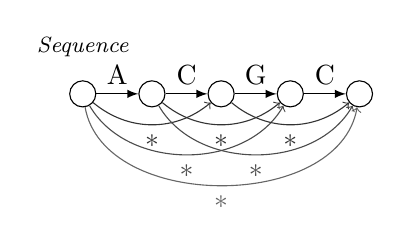
\begin{tikzpicture}[auto]
	\tikzstyle{state} = [ draw, circle, thin, node distance = 2.5em, font={\small}];
	\tikzstyle{query} = [ draw, rectangle, thin, node distance = 2.5em, font={\small}];
	\tikzstyle{info} = [font={\itshape\footnotesize}]
	\tikzstyle{point}  = [ ->, thin, font={\small}];
	\tikzstyle{extend} = [ ->, double, font={\small}];
	\tikzstyle{trace} = [ ->, thick, dashed, bend right, font={\small} ];

	\def \seq {X,A,C,G,C}

	\foreach \x [count=\xi] in \seq {
		\ifnum 1 < \xi
			\pgfmathparse{int(\xi-1)}
			\let \li \pgfmathresult
			\node[state, right of=\li] (\xi) {};
			\draw[->, >=latex] (\li) to node{\x} (\xi);
		\else
			\node[state] (\xi) {};
		\fi
	}

	\node[info] at (0,0.6) {Sequence};

	\tikzstyle{star} = [ ->, bend right, thin, color=black ];

	\foreach \xi in {1,...,3} {
		\pgfmathparse{int(\xi+2)}
		\let \xinext \pgfmathresult
		\foreach \yi in {\xinext,...,5} {
			\pgfmathparse{int(\yi - \xi)}
			\let \df \pgfmathresult
			\pgfmathparse{-\df*20}
			\let \out \pgfmathresult
			\pgfmathparse{int(180 - \out)}
			\let \in \pgfmathresult
			\pgfmathparse{int(100-\df*10)}
			\let \shade \pgfmathresult
			\draw[star, out=\out, in=\in, color=black!\shade] (\xi) to node[below]{$*$} (\yi);
		}
	}

\end{tikzpicture}
